

\documentclass[a4paper,10pt]{report}\usepackage[]{graphicx}\usepackage[]{color}
%% maxwidth is the original width if it is less than linewidth
%% otherwise use linewidth (to make sure the graphics do not exceed the margin)
\makeatletter
\def\maxwidth{ %
  \ifdim\Gin@nat@width>\linewidth
    \linewidth
  \else
    \Gin@nat@width
  \fi
}
\makeatother

\definecolor{fgcolor}{rgb}{0.345, 0.345, 0.345}
\newcommand{\hlnum}[1]{\textcolor[rgb]{0.686,0.059,0.569}{#1}}%
\newcommand{\hlstr}[1]{\textcolor[rgb]{0.192,0.494,0.8}{#1}}%
\newcommand{\hlcom}[1]{\textcolor[rgb]{0.678,0.584,0.686}{\textit{#1}}}%
\newcommand{\hlopt}[1]{\textcolor[rgb]{0,0,0}{#1}}%
\newcommand{\hlstd}[1]{\textcolor[rgb]{0.345,0.345,0.345}{#1}}%
\newcommand{\hlkwa}[1]{\textcolor[rgb]{0.161,0.373,0.58}{\textbf{#1}}}%
\newcommand{\hlkwb}[1]{\textcolor[rgb]{0.69,0.353,0.396}{#1}}%
\newcommand{\hlkwc}[1]{\textcolor[rgb]{0.333,0.667,0.333}{#1}}%
\newcommand{\hlkwd}[1]{\textcolor[rgb]{0.737,0.353,0.396}{\textbf{#1}}}%

\usepackage{framed}
\makeatletter
\newenvironment{kframe}{%
 \def\at@end@of@kframe{}%
 \ifinner\ifhmode%
  \def\at@end@of@kframe{\end{minipage}}%
  \begin{minipage}{\columnwidth}%
 \fi\fi%
 \def\FrameCommand##1{\hskip\@totalleftmargin \hskip-\fboxsep
 \colorbox{shadecolor}{##1}\hskip-\fboxsep
     % There is no \\@totalrightmargin, so:
     \hskip-\linewidth \hskip-\@totalleftmargin \hskip\columnwidth}%
 \MakeFramed {\advance\hsize-\width
   \@totalleftmargin\z@ \linewidth\hsize
   \@setminipage}}%
 {\par\unskip\endMakeFramed%
 \at@end@of@kframe}
\makeatother

\definecolor{shadecolor}{rgb}{.97, .97, .97}
\definecolor{messagecolor}{rgb}{0, 0, 0}
\definecolor{warningcolor}{rgb}{1, 0, 1}
\definecolor{errorcolor}{rgb}{1, 0, 0}
\newenvironment{knitrout}{}{} % an empty environment to be redefined in TeX

\usepackage{alltt}
\usepackage[utf8]{inputenc}
\usepackage{fontenc}
\usepackage{graphicx}
\usepackage[hidelinks]{hyperref}
\usepackage[all]{hypcap}
\usepackage{fancyhdr}
\pagestyle{fancy}
\usepackage{caption}
\usepackage{subcaption}
\usepackage{amsmath}

\date{\today}
\IfFileExists{upquote.sty}{\usepackage{upquote}}{}
\begin{document}






% Title Page
\begin{titlepage}
\begin{center}
% Title

\textsc{\Large SPM4450: Fundamentals of Data Analytics - Final Assignment Report }\\[6cm]

{ \bfseries \Large Performance of various Data Analytics Techniques on Kaggle's Problem Set `Titanic: Machine Learning from Disaster' \\[6cm] }

% Author and supervisor
\begin{minipage}{0.6\textwidth}
\emph{Authors:}\\
\begin{flushleft} \large
Nidhi \textsc{Singh}\\
4242246 \\
n.singh-2@student.tudelft.nl\\
MSc. Computer Science\\
\end{flushleft}

\begin{flushright} \large
Krishna Chaitanya \textsc{Akundi}\\
4239008 \\
k.c.akundi@student.tudelft.nl\\
MSc. Computer Science\\
\end{flushright}

\end{minipage}

\end{center}
\end{titlepage}

\listoffigures

\chapter{Titanic Data Set}
\section{Problem Description}
For our final assignment, we have taken up a challenge from Kaggle `Predict survival on the Titanic'. The dataset includes details of people who travelled on RMS Titanic which sank in 1912 killing 1502 out of 2224 passengers.
The aim of the Kaggle challenge is to complete the analysis of what sorts of people were likely to survive. In order to do so, we will apply different predictive models to the dataset and will finally evaluate their performance against each other. Kaggle also supports Leaderboards which evaluate the submitted results, but since this evaluation is based on only 50\% of the test data, it makes sense to do performance evaluation of all the models.

\ Since we are given both training and test data set, this problem's predictive models will fall under the umbrella of Supervised Learning Algorithms. Also we have to decide whether a passenger survived or not, this makes it a classic Classification problem.

\section{Data Exploration}
Before diving deep into prediction making on test data, we will explore the dataset. We are given two sets of data, training (data containing attributes and known outcomes [survived or perished] for a subset of the passengers) and test (data containing attributes without outcomes for a subset of passengers).The given training data set has 891 observations of following 12 variables:
\begin{itemize}
  \item PassengerId - Unique generated Id for each passenger
  \item Survived - Survival(0 = No; 1 = Yes)
  \item Pclass - Passenger Class (1 = 1st; 2 = 2nd; 3 = 3rd)
  \item Name - Name of the person
  \item sex - Sex 
  \item Age - Age
  \item Sibsp - Number of Siblings/Spouses Aboard
  \item Parch - Number of Parents/Children Aboard
  \item Ticket - Ticket Number
  \item Fare - Passenger Fare
  \item Cabin - Cabin in the ship
  \item Embarked - Port of Embarkation (C = Cherbourg; Q = Queenstown; S = Southampton)
  
\end{itemize}


Let us start by looking at the type of these variables
\begin{knitrout}
\definecolor{shadecolor}{rgb}{0.969, 0.969, 0.969}\color{fgcolor}\begin{kframe}
\begin{verbatim}
## 'data.frame':	891 obs. of  12 variables:
##  $ PassengerId: int  1 2 3 4 5 6 7 8 9 10 ...
##  $ Survived   : int  0 1 1 1 0 0 0 0 1 1 ...
##  $ Pclass     : int  3 1 3 1 3 3 1 3 3 2 ...
##  $ Name       : Factor w/ 891 levels "Abbing, Mr. Anthony",..: 109 191 358 277 16 559 520 629 416 581 ...
##  $ Sex        : Factor w/ 2 levels "female","male": 2 1 1 1 2 2 2 2 1 1 ...
##  $ Age        : num  22 38 26 35 35 NA 54 2 27 14 ...
##  $ SibSp      : int  1 1 0 1 0 0 0 3 0 1 ...
##  $ Parch      : int  0 0 0 0 0 0 0 1 2 0 ...
##  $ Ticket     : Factor w/ 681 levels "110152","110413",..: 525 596 662 50 473 276 86 396 345 133 ...
##  $ Fare       : num  7.25 71.28 7.92 53.1 8.05 ...
##  $ Cabin      : Factor w/ 148 levels "","A10","A14",..: 1 83 1 57 1 1 131 1 1 1 ...
##  $ Embarked   : Factor w/ 4 levels "","C","Q","S": 4 2 4 4 4 3 4 4 4 2 ...
\end{verbatim}
\end{kframe}
\end{knitrout}
Here Factor refers to categorical data, since all the names are unique, we have 891 levels equal to number of observations.
\begin{knitrout}
\definecolor{shadecolor}{rgb}{0.969, 0.969, 0.969}\color{fgcolor}\begin{kframe}
\begin{alltt}
\hlkwd{prop.table}\hlstd{(}\hlkwd{table}\hlstd{(train_csv}\hlopt{$}\hlstd{Survived))}
\end{alltt}
\begin{verbatim}
## 
##      0      1 
## 0.6162 0.3838
\end{verbatim}
\end{kframe}
\end{knitrout}
This shows that 61.6\% of the passengers perished and only 38.3\% survived.
Running the same code for Sex, we find 35.2\% females and 64.7\% in the training data set.

\begin{knitrout}
\definecolor{shadecolor}{rgb}{0.969, 0.969, 0.969}\color{fgcolor}\begin{kframe}
\begin{alltt}
\hlkwd{summary}\hlstd{(train_csv}\hlopt{$}\hlstd{Age)}
\end{alltt}
\begin{verbatim}
##    Min. 1st Qu.  Median    Mean 3rd Qu.    Max.    NA's 
##    0.42   20.10   28.00   29.70   38.00   80.00     177
\end{verbatim}
\end{kframe}
\end{knitrout}
Summary results on Age shows that this variable is missing for 177 passengers and the minimum age is 0.42 or 5 months and maximum is 80, while 90\% of the passengers were below 50.
\begin{knitrout}
\definecolor{shadecolor}{rgb}{0.969, 0.969, 0.969}\color{fgcolor}\begin{kframe}
\begin{alltt}
\hlkwd{prop.table}\hlstd{(}\hlkwd{table}\hlstd{(train_csv}\hlopt{$}\hlstd{Pclass))}
\end{alltt}
\begin{verbatim}
## 
##      1      2      3 
## 0.2424 0.2065 0.5511
\end{verbatim}
\end{kframe}
\end{knitrout}
More than 55\% passengers were travelling in third class. It will be worthwhile to see the age and sex of people in each class. 





\begin{figure}[h]
\centering
  \begin{subfigure}[b]{0.3\textwidth}
    \includegraphics[width=\textwidth]{DA-ClassBySex}
    \caption{Passenger Class by Gender.} \label{ClassBySex}
  \end{subfigure}
  \begin{subfigure}[b]{0.3\textwidth}
    \includegraphics[width=\textwidth]{DA-ClassByAge}
    \caption{Passenger Class by Age.} \label{ClassByAge}
  \end{subfigure}
  \begin{subfigure}[b]{0.3\textwidth}
    \includegraphics[width=\textwidth]{DA-ClassByFare}
    \caption{Passenger Class by Fare.} \label{ClassByFare}
  \end{subfigure}
  \caption{Passenger class by Sex, Age and Fare}\label{Class}
\end{figure}
We see in Figure\ref{Class} that third class has mostly males, since third class cabins were at the bottom of the ship this might be one of the reasons that most of the males could not survive. Also passengers in third class were younger with median below 25.With just one outlier above \$500 for first class ticket fare, fare is below \$100.





\begin{figure}[h]
\centering
  \begin{subfigure}[b]{0.3\textwidth}
    \includegraphics[width=\textwidth]{DA-Sibsp}
    \end{subfigure}
  \begin{subfigure}[b]{0.3\textwidth}
    \includegraphics[width=\textwidth]{DA-Parch}
    \end{subfigure}
  \begin{subfigure}[b]{0.3\textwidth}
    \includegraphics[width=\textwidth]{DA-Embark}
  \end{subfigure}
  \caption{Frequency of Sibsp, Parch and Embarkment}\label{Var}
\end{figure}
We now look at other variables to see if they can have some influence on predictions. From Figure \ref{Var} we can see that  most passengers travelled alone and started their journey from Southampton.

\ Other varibales `Ticket' and `Cabin' do not tell much as they have unique values, and are un-related to other variables.
\subsection{Survived variable with other variables}
Till now we looked at the variables and their values and frequencies and tried to get an initial understanding of the data.
Since we have to predict the `Survived' variable for the test set, in this section we will look at the relation between `Survived' variable and other variables.

As we can see from Figure \ref{Surv} age and fare doesnt seem to give much information about the survived variable, moreover most of the passengers were from Southampton so Place of Embarkment doesn't seem to play much role too.

But from Figure \ref{SurvCSE} we can find some interesting facts, people in 1st class outnumbered the people from 3rd class in survival rate.So there was a clear preference for elite poeple. From the second plot in Figure\ref{SurvCSE} we can see another preference was for females, we would like to believe that there was preference for children but this is not yet evident from our data. The last plot in Figure \ref{SurvCSE} shows that surely there was a clear bias for females in 1st and 2nd class compared to males. This is a clear indicator that `Sex' variable is hihgly important for our analysis with maybe `Pclass' coming next.



\begin{figure}[h]
\centering
  \begin{subfigure}[b]{0.3\textwidth}
    \includegraphics[width=\textwidth]{DA-SurvAge}
    \end{subfigure}
  \begin{subfigure}[b]{0.3\textwidth}
    \includegraphics[width=\textwidth]{DA-SurvFare}
    \end{subfigure}
    \begin{subfigure}[b]{0.3\textwidth}
    \includegraphics[width=\textwidth]{DA-SurvEmb}
  \end{subfigure}
  \caption{Passengers Survived by Age, Fare and Place of Embarkment}\label{Surv}
\end{figure}






\begin{figure}[h]
\centering
  \begin{subfigure}[b]{0.3\textwidth}
    \includegraphics[width=\textwidth]{DA-SurvClass}
    \end{subfigure}
  \begin{subfigure}[b]{0.3\textwidth}
    \includegraphics[width=\textwidth]{DA-SurvSex}
    \end{subfigure}
  \begin{subfigure}[b]{0.3\textwidth}
    \includegraphics[width=\textwidth]{DA-SurvSC}
  \end{subfigure}
  \caption{Passengers survived by Class and Gender}\label{SurvCSE}
\end{figure}

\section{Feature Engineering}
There are few variables which have `NA' and missing values, before we run our prediction models we need to get rid of these. There are 177 records in the dataset where age value is NA. For these records, we assume the age to be the average age of the group.
\subsection{Title}
The title a passenger holds, such as 'Mister', 'Miss' and others, might be a useful bit of information for predicting the fate of the passenger. To get the title from the name field, part of the name string is extracted. Also, groups of similar titles are agglomerated into a single title. 


\subsection{FamilySize}
Based on the assumption that larger families might have had trouble finding each other and getting to the lifeboats, we created a feature FamilySize which combines the SibSp and Parch features already available.

\subsection{FamilyID}
Continuing on the basis of the same assumption, we felt it would be useful to have a feature that combines family size and surname, so we can observe how large families are affected. 


\subsection{Training Data}
The training dataset containing 891 records was further partitioned with 80\% of it taken as the training set, and the remaining 20\% as the test set, to evaluate the performance of the models. So there were 713 records in the training partition and 178 records in the test partition.

\chapter{Prediction Models}
Since the `Predict survival on the Titanic' challenge is a classification problem, we will start with Linear Classifiers and then go further with methods like Decision trees and Ensembles of classifiers. In the following sections we will explore each model in detail and will also report its evaluation on Kaggle.

\section{Logistic Regression}
Logistic Regression is a classical Classification algorithm. R's \emph{glm} function is used to fit generalized linear models, With \emph{family} variable set to "binomial", glm( ) produces a logistic regression.The output of a linear regression can be transformed to a logit functions as follows:

$$
logit{p} = \log{o} = \log{p/1-p} = \beta_{0} + \beta_{1}x_{1} +\beta_{2}x_{2} + ...+\beta_{k}x_{k}
$$

Exponentiating this we get,
$$ \exp^{logit{p}} = \exp^{\beta_{0}} \exp^{\beta_{1}x_{1}} \exp^{\beta_{2}x_{2}}... \exp^{\beta_{k}x_{k}} $$
rewriting we get,
$$ o = p/1-p = \exp^{\beta_{0}} \exp^{\beta_{1}x_{1}} \exp^{\beta_{2}x_{2}}... \exp^{\beta_{k}x_{k}} $$
Here \emph{o} represents the \emph{odds}. From this we can say that if we know that a certain fact is true of a data point, then that will produce a constant change in the odds of the outcome.

We will run our first regression model with basic features provided within the dataset and can look at the results by calling summary on this model.Summary gives the value of \emph{estimated coefficients alongwith their standard errors and p-value} of each input variable. 

\begin{knitrout}
\definecolor{shadecolor}{rgb}{0.969, 0.969, 0.969}\color{fgcolor}\begin{kframe}
\begin{alltt}
\hlstd{logit.m1} \hlkwb{<-} \hlkwd{glm}\hlstd{(Survived} \hlopt{~} \hlstd{Pclass} \hlopt{+} \hlstd{Sex} \hlopt{+} \hlstd{Age} \hlopt{+} \hlstd{SibSp} \hlopt{+}
                  \hlstd{Parch} \hlopt{+} \hlstd{Fare} \hlopt{+} \hlstd{Embarked,}
                \hlkwc{data} \hlstd{= train.batch,}
                \hlkwc{family}\hlstd{=}\hlstr{"binomial"}\hlstd{)}
\hlkwd{summary}\hlstd{(logit.m1)}
\end{alltt}
\begin{verbatim}
## 
## Call:
## glm(formula = Survived ~ Pclass + Sex + Age + SibSp + Parch + 
##     Fare + Embarked, family = "binomial", data = train.batch)
## 
## Deviance Residuals: 
##    Min      1Q  Median      3Q     Max  
## -2.325  -0.617  -0.430   0.631   2.426  
## 
## Coefficients:
##             Estimate Std. Error z value Pr(>|z|)    
## (Intercept)  5.17351    0.62955    8.22  < 2e-16 ***
## Pclass      -1.06431    0.16184   -6.58  4.8e-11 ***
## Sexmale     -2.65191    0.21986  -12.06  < 2e-16 ***
## Age         -0.04189    0.00881   -4.76  2.0e-06 ***
## SibSp       -0.34715    0.11884   -2.92   0.0035 ** 
## Parch       -0.06922    0.13855   -0.50   0.6174    
## Fare         0.00301    0.00271    1.11   0.2658    
## EmbarkedQ   -0.00725    0.41417   -0.02   0.9860    
## EmbarkedS   -0.39828    0.26465   -1.50   0.1323    
## ---
## Signif. codes:  
## 0 '***' 0.001 '**' 0.01 '*' 0.05 '.' 0.1 ' ' 1
## 
## (Dispersion parameter for binomial family taken to be 1)
## 
##     Null deviance: 951.76  on 712  degrees of freedom
## Residual deviance: 634.98  on 704  degrees of freedom
## AIC: 653
## 
## Number of Fisher Scoring iterations: 5
\end{verbatim}
\end{kframe}
\end{knitrout}

Logistic Regression uses the deviance test to estimate the goodness of the model. Its approach is based on estimating two models, it assumes that one excludes the hypothesized effects to be null, while to be included in 
the other. For each model, a deviance statistic, equal to -2 ln L for that model, is computed, which in this case is
\emph{951.76(Null model) and 634.98(estimated model)}. The deviance can be regarded as a measure of lack of fit between 
model and data. In general, the larger the deviance, the poorer the fit to the data. In our first iteration with basic
features we can see reduction of \emph{316.78} in deviance. The difference between the deviances has a large-sample chi-square distribution with degrees of freedom equal to the difference in the number of parameters estimated. Thus the difference in deviances can be tested against the chi-square distribution for significance, as done below.

\begin{knitrout}
\definecolor{shadecolor}{rgb}{0.969, 0.969, 0.969}\color{fgcolor}\begin{kframe}
\begin{alltt}
\hlkwd{pchisq}\hlstd{(}\hlnum{951.76}\hlopt{-}\hlnum{634.98}\hlstd{,} \hlnum{8}\hlstd{)}
\end{alltt}
\begin{verbatim}
## [1] 1
\end{verbatim}
\end{kframe}
\end{knitrout}
Also, we can see from the summary that only \emph{Pclass, Sex, Age and SibSp(moderately)} has effect on the model with significance less than .05 level. To see how these variables affect, we can also do \emph{ANOVA} test, which tries adding the factors in the given order.
\begin{knitrout}
\definecolor{shadecolor}{rgb}{0.969, 0.969, 0.969}\color{fgcolor}\begin{kframe}
\begin{alltt}
\hlkwd{anova}\hlstd{(logit.m1,} \hlkwc{test}\hlstd{=}\hlstr{"Chisq"}\hlstd{)}
\end{alltt}
\begin{verbatim}
## Analysis of Deviance Table
## 
## Model: binomial, link: logit
## 
## Response: Survived
## 
## Terms added sequentially (first to last)
## 
## 
##          Df Deviance Resid. Df Resid. Dev Pr(>Chi)    
## NULL                       712        952             
## Pclass    1     80.1       711        872  < 2e-16 ***
## Sex       1    198.9       710        673  < 2e-16 ***
## Age       1     19.4       709        653  1.1e-05 ***
## SibSp     1     12.8       708        641  0.00035 ***
## Parch     1      0.1       707        640  0.79638    
## Fare      1      2.4       706        638  0.12427    
## Embarked  2      3.1       704        635  0.20912    
## ---
## Signif. codes:  
## 0 '***' 0.001 '**' 0.01 '*' 0.05 '.' 0.1 ' ' 1
\end{verbatim}
\end{kframe}
\end{knitrout}
From the ANOVA results too, we can see that the deviance is highly reduced by \emph{Pclass, Sex} and weakly reduced by \emph{Age and SibSp} and with more or less no affect on deviance by other variables(Parch, Fare and Embarked).
To improve our model further we can make use of \emph{engineered variables} from previous chapter, namely \emph{Title,FamilySize and FamilyID2}

\begin{knitrout}
\definecolor{shadecolor}{rgb}{0.969, 0.969, 0.969}\color{fgcolor}\begin{kframe}
\begin{alltt}
\hlstd{logit.m2} \hlkwb{<-} \hlkwd{glm}\hlstd{(Survived} \hlopt{~} \hlstd{Pclass} \hlopt{+} \hlstd{Sex} \hlopt{+} \hlstd{Age} \hlopt{+} \hlstd{SibSp} \hlopt{+} \hlstd{Parch} \hlopt{+}
                  \hlstd{Embarked} \hlopt{+} \hlstd{Title} \hlopt{+}
                  \hlstd{FamilyID2,}
                \hlkwc{data} \hlstd{= train.batch,}
                \hlkwc{family}\hlstd{=}\hlstr{"binomial"}\hlstd{)}
\hlkwd{summary}\hlstd{(logit.m2)}
\hlkwd{pchisq}\hlstd{(}\hlnum{406.25}\hlstd{,} \hlnum{36}\hlstd{)}
\hlkwd{anova}\hlstd{(logit.m2,} \hlkwc{test}\hlstd{=}\hlstr{"Chisq"}\hlstd{)}
\end{alltt}
\end{kframe}
\end{knitrout}

The new model results in \emph{545.51} deviance, reducing \emph{406.25} points over null deviance of 951.76. The ANOVA test results show that the engineered variable \emph{Title and FamilyID2} have a significant effect on deviance. Thus, we will be including it in our further modelling.

We can now see how the new model performs on the test data.

\begin{knitrout}
\definecolor{shadecolor}{rgb}{0.969, 0.969, 0.969}\color{fgcolor}\begin{kframe}
\begin{alltt}
\hlkwd{confusionMatrix}\hlstd{(logit.predict.val, test.batch}\hlopt{$}\hlstd{Survived)}
\end{alltt}
\begin{verbatim}
## Confusion Matrix and Statistics
## 
##           Reference
## Prediction   0   1
##          0 102  15
##          1  10  51
##                                       
##                Accuracy : 0.86        
##                  95% CI : (0.8, 0.907)
##     No Information Rate : 0.629       
##     P-Value [Acc > NIR] : 7.64e-12    
##                                       
##                   Kappa : 0.694       
##  Mcnemar's Test P-Value : 0.424       
##                                       
##             Sensitivity : 0.911       
##             Specificity : 0.773       
##          Pos Pred Value : 0.872       
##          Neg Pred Value : 0.836       
##              Prevalence : 0.629       
##          Detection Rate : 0.573       
##    Detection Prevalence : 0.657       
##       Balanced Accuracy : 0.842       
##                                       
##        'Positive' Class : 0           
## 
\end{verbatim}
\end{kframe}
\end{knitrout}
This model does well based on accuracy

\section{Naive Bayes}
Naive Bayes (NB) and Logistic Regression are both linear classifiers but they estimate parameters differently. Logistic Regression estimates the best model fit by minimizing the error or deviances, whereas Naive Bayes estimates `prior' probability from the training data and uses Bayes rule to predict new instances.

Since our training set has fewer instances, logistic regression might overfit, thus it would be interesting to see the performance of Naive Bayes. Also with Naive Bayes an assumption is made that our inputs are independent, thus we should not have collinear inputs in our model.
\begin{knitrout}
\definecolor{shadecolor}{rgb}{0.969, 0.969, 0.969}\color{fgcolor}\begin{kframe}
\begin{alltt}
\hlstd{nb.classifier} \hlkwb{<-} \hlkwd{naiveBayes}\hlstd{(}\hlkwd{as.factor}\hlstd{(Survived)} \hlopt{~} \hlstd{Pclass} \hlopt{+} \hlstd{Sex} \hlopt{+}
                   \hlstd{Age} \hlopt{+} \hlstd{SibSp} \hlopt{+} \hlstd{Parch} \hlopt{+} \hlstd{Embarked} \hlopt{+}
                   \hlstd{Title} \hlopt{+} \hlstd{FamilyID2,}
                  \hlkwc{data} \hlstd{= train.batch)}
\hlstd{nb.predict} \hlkwb{<-} \hlkwd{predict}\hlstd{(nb.classifier, test.batch)}
\end{alltt}


{\ttfamily\noindent\color{warningcolor}{\#\# Warning: NAs introduced by coercion\\\#\# Warning: NAs introduced by coercion}}\end{kframe}
\end{knitrout}
To see the accuracy of the NB model on test data set, we can look at confusion matrix statistics
\begin{knitrout}
\definecolor{shadecolor}{rgb}{0.969, 0.969, 0.969}\color{fgcolor}\begin{kframe}
\begin{alltt}
\hlkwd{confusionMatrix}\hlstd{(nb.predict,test.batch}\hlopt{$}\hlstd{Survived)}
\end{alltt}
\begin{verbatim}
## Confusion Matrix and Statistics
## 
##           Reference
## Prediction  0  1
##          0 98 17
##          1 14 49
##                                         
##                Accuracy : 0.826         
##                  95% CI : (0.762, 0.878)
##     No Information Rate : 0.629         
##     P-Value [Acc > NIR] : 7.85e-09      
##                                         
##                   Kappa : 0.623         
##  Mcnemar's Test P-Value : 0.719         
##                                         
##             Sensitivity : 0.875         
##             Specificity : 0.742         
##          Pos Pred Value : 0.852         
##          Neg Pred Value : 0.778         
##              Prevalence : 0.629         
##          Detection Rate : 0.551         
##    Detection Prevalence : 0.646         
##       Balanced Accuracy : 0.809         
##                                         
##        'Positive' Class : 0             
## 
\end{verbatim}
\end{kframe}
\end{knitrout}

The NB model performs with 82.6\% accuracy on test batch but performs poorly and same as Logistic Regression on Kaggle test batch with 77.03\% accuracy.

\section{Decision Trees}
Decision tree algorithms work by repeatedly splitting the dataset into subsets based on a particular attribute value. This process is recursively carried out until further splitting does not add any value to the predictions. This is a greedy algorithm, which means that decisions with the highest immediate value are given preference.

We applied recursive partitioning on the Titanic dataset using the Decision Tree algorithm from R's \emph{rpart} package . For this, the dependent variables used were Pclass, Sex, Age, Fare, Embarked, Title and FamilyID2. 

The algorithm was run multiple times with different control parameters, and then analyzed the results through a confusion matrix. We used the same set of features over these runs - Pclass, Sex, Age, SibSp, Parch, Embarked, Title and FamilyID2.
\subsection{}
We first ran the rpart algorithm using a minsplit value of 2 and complexity parameter of 0.01.
\begin{knitrout}
\definecolor{shadecolor}{rgb}{0.969, 0.969, 0.969}\color{fgcolor}\begin{kframe}
\begin{alltt}
\hlstd{dt.1} \hlkwb{<-} \hlkwd{rpart}\hlstd{(Survived} \hlopt{~} \hlstd{Pclass} \hlopt{+} \hlstd{Sex} \hlopt{+} \hlstd{Age} \hlopt{+} \hlstd{SibSp} \hlopt{+} \hlstd{Parch} \hlopt{+}
    \hlstd{Embarked} \hlopt{+} \hlstd{Title} \hlopt{+} \hlstd{FamilyID2,} \hlkwc{data} \hlstd{= train.batch,} \hlkwc{method} \hlstd{=} \hlstr{"class"}\hlstd{,}
    \hlkwc{control} \hlstd{=} \hlkwd{rpart.control}\hlstd{(}\hlkwc{minsplit} \hlstd{=} \hlnum{2}\hlstd{,} \hlkwc{cp} \hlstd{=} \hlnum{0.01}\hlstd{))}
\hlstd{dt.1.pred} \hlkwb{<-} \hlkwd{predict}\hlstd{(dt.1, test.batch,} \hlkwc{type} \hlstd{=} \hlstr{"class"}\hlstd{)}
\hlkwd{confusionMatrix}\hlstd{(dt.1.pred, test.batch}\hlopt{$}\hlstd{Survived)}
\end{alltt}
\begin{verbatim}
## Confusion Matrix and Statistics
## 
##           Reference
## Prediction   0   1
##          0 107  28
##          1   5  38
##                                        
##                Accuracy : 0.815        
##                  95% CI : (0.75, 0.869)
##     No Information Rate : 0.629        
##     P-Value [Acc > NIR] : 5.78e-08     
##                                        
##                   Kappa : 0.572        
##  Mcnemar's Test P-Value : 0.000128     
##                                        
##             Sensitivity : 0.955        
##             Specificity : 0.576        
##          Pos Pred Value : 0.793        
##          Neg Pred Value : 0.884        
##              Prevalence : 0.629        
##          Detection Rate : 0.601        
##    Detection Prevalence : 0.758        
##       Balanced Accuracy : 0.766        
##                                        
##        'Positive' Class : 0            
## 
\end{verbatim}
\end{kframe}
\end{knitrout}

Here, the first parameter indicates the formula for the dependent variable being estimated with respect to the independent variables, the second indicates the training data set, the third indicates the method, which is set to 'class' as the variable 'Survived' has only two levels. The last argument specifies various parameters for the working of the recursive partitioning algorithm. In our case, we specify 'minsplit', which indicates the minimum number of observations required at a node to make a split. \emph{cp} is the complexity parameter. Any split that does not reduce complexity by a factor of \emph{cp} is not made. This resulted in a model which predicted the correct outcome 76.55\% of the time.
\begin{figure}[h]
  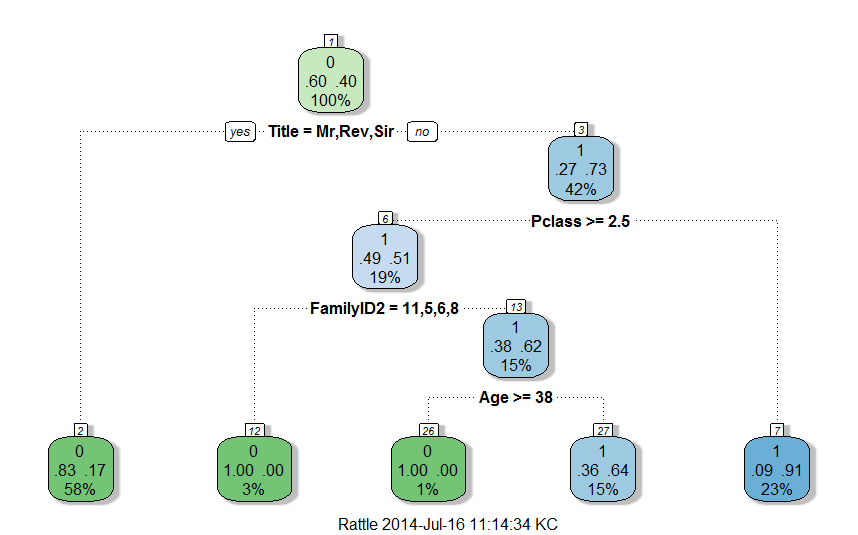
\includegraphics[width=\textwidth]{dt1}
  \caption{Decision tree with minsplit=2 and complex parameter=.01} \label{dt1}
\end{figure}

\subsection{}
In the second run, we added control parameters which specified \emph{minsplit} as 2 and \emph{cp} as 0. This allowed unbounded growth for the tree.
\begin{knitrout}
\definecolor{shadecolor}{rgb}{0.969, 0.969, 0.969}\color{fgcolor}\begin{kframe}
\begin{alltt}
\hlstd{dt.2} \hlkwb{<-} \hlkwd{rpart}\hlstd{(Survived} \hlopt{~} \hlstd{Pclass} \hlopt{+} \hlstd{Sex} \hlopt{+} \hlstd{Age} \hlopt{+} \hlstd{SibSp} \hlopt{+} \hlstd{Parch} \hlopt{+}
    \hlstd{Embarked} \hlopt{+} \hlstd{Title} \hlopt{+} \hlstd{FamilyID2,} \hlkwc{data} \hlstd{= train.batch,} \hlkwc{method} \hlstd{=} \hlstr{"class"}\hlstd{,}
    \hlkwc{control} \hlstd{=} \hlkwd{rpart.control}\hlstd{(}\hlkwc{minsplit} \hlstd{=} \hlnum{2}\hlstd{,} \hlkwc{cp} \hlstd{=} \hlnum{0}\hlstd{))}
\hlstd{dt.2.pred} \hlkwb{<-} \hlkwd{predict}\hlstd{(dt.2, test.batch,} \hlkwc{type} \hlstd{=} \hlstr{"class"}\hlstd{)}
\hlkwd{confusionMatrix}\hlstd{(dt.2.pred, test.batch}\hlopt{$}\hlstd{Survived)}
\end{alltt}
\begin{verbatim}
## Confusion Matrix and Statistics
## 
##           Reference
## Prediction  0  1
##          0 97 17
##          1 15 49
##                                         
##                Accuracy : 0.82          
##                  95% CI : (0.756, 0.874)
##     No Information Rate : 0.629         
##     P-Value [Acc > NIR] : 2.17e-08      
##                                         
##                   Kappa : 0.612         
##  Mcnemar's Test P-Value : 0.86          
##                                         
##             Sensitivity : 0.866         
##             Specificity : 0.742         
##          Pos Pred Value : 0.851         
##          Neg Pred Value : 0.766         
##              Prevalence : 0.629         
##          Detection Rate : 0.545         
##    Detection Prevalence : 0.640         
##       Balanced Accuracy : 0.804         
##                                         
##        'Positive' Class : 0             
## 
\end{verbatim}
\end{kframe}
\end{knitrout}
We ended up with a complex structure with large a number of branches. However, there were no significant gains in accuracy, sensitivity or precision. This model predicted outcomes for unseen data correctly in 71.29\% of cases. 

\begin{figure}[h]
  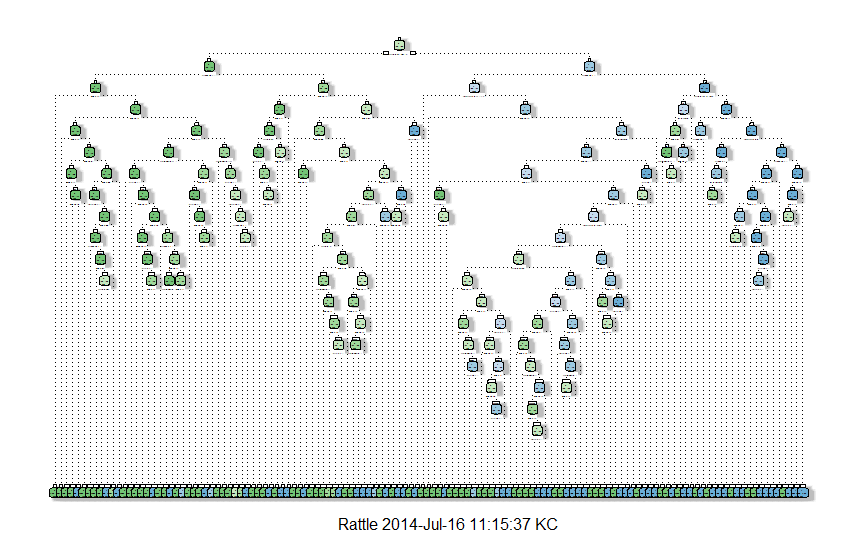
\includegraphics[width=\textwidth]{dt2}
  \caption{Decision tree with minsplit=2 and complex parameter as 0} \label{dt2}
\end{figure}
\subsection{}
In the last run, we specified \emph{minsplit} as 16 and \emph{cp} as 0.001.
\begin{knitrout}
\definecolor{shadecolor}{rgb}{0.969, 0.969, 0.969}\color{fgcolor}\begin{kframe}
\begin{alltt}
\hlstd{dt.3} \hlkwb{<-} \hlkwd{rpart}\hlstd{(Survived} \hlopt{~} \hlstd{Pclass} \hlopt{+} \hlstd{Sex} \hlopt{+} \hlstd{Age} \hlopt{+} \hlstd{SibSp} \hlopt{+} \hlstd{Parch} \hlopt{+}
    \hlstd{Embarked} \hlopt{+} \hlstd{Title} \hlopt{+} \hlstd{FamilyID2,} \hlkwc{data} \hlstd{= train.batch,} \hlkwc{method} \hlstd{=} \hlstr{"class"}\hlstd{,}
    \hlkwc{control} \hlstd{=} \hlkwd{rpart.control}\hlstd{(}\hlkwc{minsplit} \hlstd{=} \hlnum{16}\hlstd{,} \hlkwc{cp} \hlstd{=} \hlnum{0.001}\hlstd{))}
\hlstd{dt.3.pred} \hlkwb{<-} \hlkwd{predict}\hlstd{(dt.3, test.batch,} \hlkwc{type} \hlstd{=} \hlstr{"class"}\hlstd{)}
\hlkwd{confusionMatrix}\hlstd{(dt.3.pred, test.batch}\hlopt{$}\hlstd{Survived)}
\end{alltt}
\begin{verbatim}
## Confusion Matrix and Statistics
## 
##           Reference
## Prediction   0   1
##          0 103  22
##          1   9  44
##                                         
##                Accuracy : 0.826         
##                  95% CI : (0.762, 0.878)
##     No Information Rate : 0.629         
##     P-Value [Acc > NIR] : 7.85e-09      
##                                         
##                   Kappa : 0.611         
##  Mcnemar's Test P-Value : 0.0311        
##                                         
##             Sensitivity : 0.920         
##             Specificity : 0.667         
##          Pos Pred Value : 0.824         
##          Neg Pred Value : 0.830         
##              Prevalence : 0.629         
##          Detection Rate : 0.579         
##    Detection Prevalence : 0.702         
##       Balanced Accuracy : 0.793         
##                                         
##        'Positive' Class : 0             
## 
\end{verbatim}
\end{kframe}
\end{knitrout}
The resulting model was better with respect to most metrics when it came to the training data, and did reasonably well with the test data, correctly predicting 77.09\% of the cases.
\begin{figure}[h]
  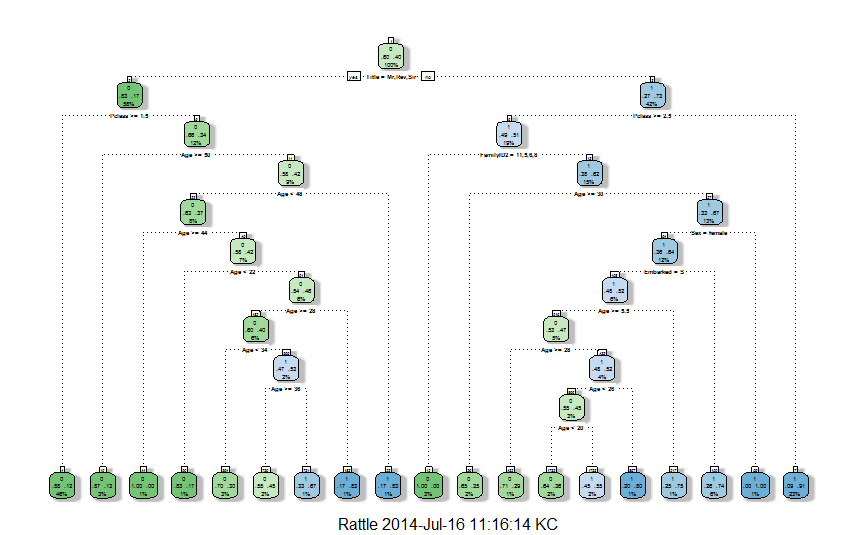
\includegraphics[width=\textwidth]{dt3}
  \caption{Decision tree with minsplit=16 and complex parameter=.001} \label{dt3}
\end{figure}
\section{Support Vector Machines}

Support Vector Machine (SVM) algorithms perform classification by representing the given data as points in space, with a clear plane of separation between the different classes to which the points belong. SVMs use the 'kernel trick' to work with high-dimensional data without ever having to map the points in such spaces. 
In R, the \texttt{e1071} and \texttt{kernlab} packages offer methods for creating SVM models. We used the \texttt{kernlab} package to generate our SVM models.

\subsection{}
Initially, the algorithm was run using all the features that were already present in the given dataset. The model performs well on the training dataset, with an accuracy of 84.27\%. However, it did not do so well on the test set, being able to predict the correct outcome only around 62\% of the time. More statistics from the tests are shown below.
\begin{knitrout}
\definecolor{shadecolor}{rgb}{0.969, 0.969, 0.969}\color{fgcolor}\begin{kframe}
\begin{alltt}
\hlstd{svm.model.1} \hlkwb{<-} \hlkwd{ksvm}\hlstd{(Survived} \hlopt{~} \hlstd{Pclass} \hlopt{+} \hlstd{Sex} \hlopt{+} \hlstd{Age} \hlopt{+} \hlstd{SibSp} \hlopt{+} \hlstd{Parch} \hlopt{+}
    \hlstd{Embarked} \hlopt{+} \hlstd{Title} \hlopt{+} \hlstd{FamilyID2,} \hlkwc{data} \hlstd{= train.batch,} \hlkwc{kernel} \hlstd{=} \hlstr{"rbfdot"}\hlstd{,}
    \hlkwc{type} \hlstd{=} \hlstr{"C-svc"}\hlstd{)}
\end{alltt}
\begin{verbatim}
## Using automatic sigma estimation (sigest) for RBF or laplace kernel
\end{verbatim}
\begin{alltt}
\hlstd{svm.pred.1} \hlkwb{<-} \hlkwd{predict}\hlstd{(svm.model.1,} \hlkwc{type} \hlstd{=} \hlstr{"response"}\hlstd{, test.batch)}
\hlkwd{confusionMatrix}\hlstd{(svm.pred.1, test.batch}\hlopt{$}\hlstd{Survived)}
\end{alltt}
\begin{verbatim}
## Confusion Matrix and Statistics
## 
##           Reference
## Prediction   0   1
##          0 106  25
##          1   6  41
##                                         
##                Accuracy : 0.826         
##                  95% CI : (0.762, 0.878)
##     No Information Rate : 0.629         
##     P-Value [Acc > NIR] : 7.85e-09      
##                                         
##                   Kappa : 0.603         
##  Mcnemar's Test P-Value : 0.00123       
##                                         
##             Sensitivity : 0.946         
##             Specificity : 0.621         
##          Pos Pred Value : 0.809         
##          Neg Pred Value : 0.872         
##              Prevalence : 0.629         
##          Detection Rate : 0.596         
##    Detection Prevalence : 0.736         
##       Balanced Accuracy : 0.784         
##                                         
##        'Positive' Class : 0             
## 
\end{verbatim}
\end{kframe}
\end{knitrout}
Here, the type 'C-svc' indicates that the algorithm must run in the classification mode.
\subsection{}
The algorithm was then run using a subset of the available features, containing Pclass, Sex and Embarked. 
\begin{knitrout}
\definecolor{shadecolor}{rgb}{0.969, 0.969, 0.969}\color{fgcolor}\begin{kframe}
\begin{alltt}
\hlstd{svm.model.2} \hlkwb{<-} \hlkwd{ksvm}\hlstd{(Survived} \hlopt{~} \hlstd{Sex} \hlopt{+} \hlstd{Pclass} \hlopt{+} \hlstd{Embarked,} \hlkwc{data} \hlstd{= train.batch,}
    \hlkwc{kernel} \hlstd{=} \hlstr{"rbfdot"}\hlstd{,} \hlkwc{type} \hlstd{=} \hlstr{"C-svc"}\hlstd{)}
\end{alltt}
\begin{verbatim}
## Using automatic sigma estimation (sigest) for RBF or laplace kernel
\end{verbatim}
\begin{alltt}
\hlstd{svm.pred.2} \hlkwb{<-} \hlkwd{predict}\hlstd{(svm.model.2,} \hlkwc{type} \hlstd{=} \hlstr{"response"}\hlstd{, test.batch)}
\hlkwd{confusionMatrix}\hlstd{(svm.pred.2, test.batch}\hlopt{$}\hlstd{Survived)}
\end{alltt}
\begin{verbatim}
## Confusion Matrix and Statistics
## 
##           Reference
## Prediction   0   1
##          0 107  31
##          1   5  35
##                                         
##                Accuracy : 0.798         
##                  95% CI : (0.731, 0.854)
##     No Information Rate : 0.629         
##     P-Value [Acc > NIR] : 8.83e-07      
##                                         
##                   Kappa : 0.528         
##  Mcnemar's Test P-Value : 3.09e-05      
##                                         
##             Sensitivity : 0.955         
##             Specificity : 0.530         
##          Pos Pred Value : 0.775         
##          Neg Pred Value : 0.875         
##              Prevalence : 0.629         
##          Detection Rate : 0.601         
##    Detection Prevalence : 0.775         
##       Balanced Accuracy : 0.743         
##                                         
##        'Positive' Class : 0             
## 
\end{verbatim}
\end{kframe}
\end{knitrout}
This model proved to be slightly better performing with the training data, with an accuracy of 84.83\%, while exhibiting higher sensitivity and lower specificity. The model performed significantly better on unseen data, correctly predicting outcomes 77.99\% of the time.

\subsection{}
In the next run, the engineered features Title and FamilyID2 were used along with Pclass and Sex to create the model.
\begin{knitrout}
\definecolor{shadecolor}{rgb}{0.969, 0.969, 0.969}\color{fgcolor}\begin{kframe}
\begin{alltt}
\hlstd{svm.model.3} \hlkwb{<-} \hlkwd{ksvm}\hlstd{(Survived} \hlopt{~} \hlstd{Sex} \hlopt{+} \hlstd{Pclass} \hlopt{+} \hlstd{Embarked} \hlopt{+} \hlstd{Title} \hlopt{+}
    \hlstd{FamilyID2,} \hlkwc{data} \hlstd{= train.batch,} \hlkwc{kernel} \hlstd{=} \hlstr{"rbfdot"}\hlstd{,} \hlkwc{type} \hlstd{=} \hlstr{"C-svc"}\hlstd{,}
    \hlkwc{prob.model} \hlstd{=} \hlnum{TRUE}\hlstd{)}
\end{alltt}
\begin{verbatim}
## Using automatic sigma estimation (sigest) for RBF or laplace kernel
\end{verbatim}
\begin{alltt}
\hlstd{svm.pred.3} \hlkwb{<-} \hlkwd{predict}\hlstd{(svm.model.3,} \hlkwc{type} \hlstd{=} \hlstr{"response"}\hlstd{, test.batch)}
\hlkwd{confusionMatrix}\hlstd{(svm.pred.3, test.batch}\hlopt{$}\hlstd{Survived)}
\end{alltt}
\begin{verbatim}
## Confusion Matrix and Statistics
## 
##           Reference
## Prediction   0   1
##          0 107  29
##          1   5  37
##                                         
##                Accuracy : 0.809         
##                  95% CI : (0.743, 0.864)
##     No Information Rate : 0.629         
##     P-Value [Acc > NIR] : 1.48e-07      
##                                         
##                   Kappa : 0.558         
##  Mcnemar's Test P-Value : 8.00e-05      
##                                         
##             Sensitivity : 0.955         
##             Specificity : 0.561         
##          Pos Pred Value : 0.787         
##          Neg Pred Value : 0.881         
##              Prevalence : 0.629         
##          Detection Rate : 0.601         
##    Detection Prevalence : 0.764         
##       Balanced Accuracy : 0.758         
##                                         
##        'Positive' Class : 0             
## 
\end{verbatim}
\end{kframe}
\end{knitrout}
This model showed slightly better performance compared to the previous one, both with the training data and the test set from Kaggle.
\subsection{}
In the final run, we constructed the SVM model using the feature set used for the other models. The performance of this model on the training set was comparable to that of the other models. On the unseen test data, the model performed well also, predicting the right outcome 78.46\% of the time.  
\begin{knitrout}
\definecolor{shadecolor}{rgb}{0.969, 0.969, 0.969}\color{fgcolor}\begin{kframe}
\begin{alltt}
\hlstd{svm.model.4} \hlkwb{<-} \hlkwd{ksvm}\hlstd{(Survived} \hlopt{~} \hlstd{Pclass} \hlopt{+} \hlstd{Sex} \hlopt{+} \hlstd{Age} \hlopt{+} \hlstd{SibSp} \hlopt{+} \hlstd{Parch} \hlopt{+}
    \hlstd{Embarked} \hlopt{+} \hlstd{Title} \hlopt{+} \hlstd{FamilyID2,} \hlkwc{data} \hlstd{= train.batch,} \hlkwc{kernel} \hlstd{=} \hlstr{"rbfdot"}\hlstd{,}
    \hlkwc{type} \hlstd{=} \hlstr{"C-svc"}\hlstd{)}
\end{alltt}
\begin{verbatim}
## Using automatic sigma estimation (sigest) for RBF or laplace kernel
\end{verbatim}
\begin{alltt}
\hlstd{svm.pred.4} \hlkwb{<-} \hlkwd{predict}\hlstd{(svm.model.4,} \hlkwc{type} \hlstd{=} \hlstr{"response"}\hlstd{, test.batch)}
\hlkwd{confusionMatrix}\hlstd{(svm.pred.4, test.batch}\hlopt{$}\hlstd{Survived)}
\end{alltt}
\begin{verbatim}
## Confusion Matrix and Statistics
## 
##           Reference
## Prediction   0   1
##          0 106  25
##          1   6  41
##                                         
##                Accuracy : 0.826         
##                  95% CI : (0.762, 0.878)
##     No Information Rate : 0.629         
##     P-Value [Acc > NIR] : 7.85e-09      
##                                         
##                   Kappa : 0.603         
##  Mcnemar's Test P-Value : 0.00123       
##                                         
##             Sensitivity : 0.946         
##             Specificity : 0.621         
##          Pos Pred Value : 0.809         
##          Neg Pred Value : 0.872         
##              Prevalence : 0.629         
##          Detection Rate : 0.596         
##    Detection Prevalence : 0.736         
##       Balanced Accuracy : 0.784         
##                                         
##        'Positive' Class : 0             
## 
\end{verbatim}
\end{kframe}
\end{knitrout}

\section{Random Forests}
Random Forests are an extension of tree methods. The inherent variability of the tree model, and susceptibility to data is a problem, in random forest this is considered a strength. The intuition is that by averaging across the high variance and low bias trees we will end up with low variance low bias estimated model. We will be using R's \texttt{randomForest} package which is based on Breiman and Cutler's original Fortran code.

Before modelling we need to decide on few input variables needed for the algorithm, the number of trees to grow, \texttt{ntree}, its value should be such that each input row should get predicted a few times. Also number of variables to be sampled as candidates at each split, \texttt{mtry}, should be decided. To find the optimal value of \texttt{mtry}, we can use \texttt{tuneRF} function of \texttt{randomForest} package.
\begin{knitrout}
\definecolor{shadecolor}{rgb}{0.969, 0.969, 0.969}\color{fgcolor}\begin{kframe}
\begin{alltt}
\hlstd{bestmtry} \hlkwb{<-} \hlkwd{tuneRF}\hlstd{(}\hlkwd{data.frame}\hlstd{(train.batch}\hlopt{$}\hlstd{Pclass,train.batch}\hlopt{$}\hlstd{Sex,}
                              \hlstd{train.batch}\hlopt{$}\hlstd{Age,train.batch}\hlopt{$}\hlstd{SibSp,}
                              \hlstd{train.batch}\hlopt{$}\hlstd{Parch,train.batch}\hlopt{$}\hlstd{Embarked,}
                              \hlstd{train.batch}\hlopt{$}\hlstd{Title,train.batch}\hlopt{$}\hlstd{FamilyID2),}
                   \hlstd{train.batch}\hlopt{$}\hlstd{Survived,} \hlkwc{ntreeTry}\hlstd{=}\hlnum{100}\hlstd{,}
                   \hlkwc{stepFactor}\hlstd{=}\hlnum{1.5}\hlstd{,}\hlkwc{improve}\hlstd{=}\hlnum{0.01}\hlstd{,} \hlkwc{trace}\hlstd{=}\hlnum{TRUE}\hlstd{,} \hlkwc{plot}\hlstd{=}\hlnum{TRUE}\hlstd{,}
                   \hlkwc{dobest}\hlstd{=}\hlnum{FALSE}\hlstd{)}
\end{alltt}
\end{kframe}
\end{knitrout}
Here \texttt{ntreeTry} is the number of trees used at the tuning step, \texttt{stepFactor} value by which mtry is inflated at every iteration. This function gives the value of \texttt{mtry} as \emph{3}. 
We now perform random forest algorithm, first with \texttt{ntree} set to 1000.
\begin{knitrout}
\definecolor{shadecolor}{rgb}{0.969, 0.969, 0.969}\color{fgcolor}\begin{kframe}
\begin{alltt}
\hlstd{rf.m1} \hlkwb{<-}\hlkwd{randomForest}\hlstd{(}\hlkwd{as.factor}\hlstd{(Survived)} \hlopt{~} \hlstd{Pclass} \hlopt{+} \hlstd{Sex} \hlopt{+} \hlstd{Age} \hlopt{+} \hlstd{SibSp} \hlopt{+}
                       \hlstd{Parch} \hlopt{+} \hlstd{Fare}\hlopt{+} \hlstd{FamilySize} \hlopt{+}
                       \hlstd{Embarked} \hlopt{+} \hlstd{Title} \hlopt{+} \hlstd{FamilyID2,}
                     \hlkwc{data}\hlstd{=train.batch,} \hlkwc{mtry}\hlstd{=}\hlnum{3}\hlstd{,} \hlkwc{ntree}\hlstd{=}\hlnum{2000}\hlstd{,}
                     \hlkwc{keep.forest}\hlstd{=}\hlnum{TRUE}\hlstd{,} \hlkwc{importance}\hlstd{=}\hlnum{TRUE}\hlstd{)}
\hlstd{rf.predict.1} \hlkwb{<-} \hlkwd{predict}\hlstd{(rf.m1, test.batch,} \hlkwc{type} \hlstd{=} \hlstr{"response"}\hlstd{)}
\hlkwd{confusionMatrix}\hlstd{(rf.predict.1, test.batch}\hlopt{$}\hlstd{Survived)}
\end{alltt}
\begin{verbatim}
## Confusion Matrix and Statistics
## 
##           Reference
## Prediction   0   1
##          0 104  21
##          1   8  45
##                                         
##                Accuracy : 0.837         
##                  95% CI : (0.774, 0.888)
##     No Information Rate : 0.629         
##     P-Value [Acc > NIR] : 9.16e-10      
##                                         
##                   Kappa : 0.636         
##  Mcnemar's Test P-Value : 0.0259        
##                                         
##             Sensitivity : 0.929         
##             Specificity : 0.682         
##          Pos Pred Value : 0.832         
##          Neg Pred Value : 0.849         
##              Prevalence : 0.629         
##          Detection Rate : 0.584         
##    Detection Prevalence : 0.702         
##       Balanced Accuracy : 0.805         
##                                         
##        'Positive' Class : 0             
## 
\end{verbatim}
\end{kframe}
\end{knitrout}
and then again with \texttt{ntree} set to 2000
\begin{knitrout}
\definecolor{shadecolor}{rgb}{0.969, 0.969, 0.969}\color{fgcolor}\begin{kframe}
\begin{alltt}
\hlstd{rf.m2} \hlkwb{<-}\hlkwd{randomForest}\hlstd{(}\hlkwd{as.factor}\hlstd{(Survived)} \hlopt{~} \hlstd{Pclass} \hlopt{+} \hlstd{Sex} \hlopt{+} \hlstd{Age} \hlopt{+} \hlstd{SibSp} \hlopt{+}
                       \hlstd{Parch} \hlopt{+} \hlstd{Fare}\hlopt{+} \hlstd{FamilySize} \hlopt{+}
                       \hlstd{Embarked} \hlopt{+} \hlstd{Title} \hlopt{+} \hlstd{FamilyID2,}
                     \hlkwc{data}\hlstd{=train.batch,} \hlkwc{mtry}\hlstd{=}\hlnum{3}\hlstd{,} \hlkwc{ntree}\hlstd{=}\hlnum{2000}\hlstd{,}
                     \hlkwc{keep.forest}\hlstd{=}\hlnum{TRUE}\hlstd{,} \hlkwc{importance}\hlstd{=}\hlnum{TRUE}\hlstd{)}
\hlstd{rf.predict.2} \hlkwb{<-} \hlkwd{predict}\hlstd{(rf.m2, test.batch,} \hlkwc{type} \hlstd{=} \hlstr{"response"}\hlstd{)}
\hlkwd{confusionMatrix}\hlstd{(rf.predict.2, test.batch}\hlopt{$}\hlstd{Survived)}
\end{alltt}
\begin{verbatim}
## Confusion Matrix and Statistics
## 
##           Reference
## Prediction   0   1
##          0 103  21
##          1   9  45
##                                         
##                Accuracy : 0.831         
##                  95% CI : (0.768, 0.883)
##     No Information Rate : 0.629         
##     P-Value [Acc > NIR] : 2.73e-09      
##                                         
##                   Kappa : 0.625         
##  Mcnemar's Test P-Value : 0.0446        
##                                         
##             Sensitivity : 0.920         
##             Specificity : 0.682         
##          Pos Pred Value : 0.831         
##          Neg Pred Value : 0.833         
##              Prevalence : 0.629         
##          Detection Rate : 0.579         
##    Detection Prevalence : 0.697         
##       Balanced Accuracy : 0.801         
##                                         
##        'Positive' Class : 0             
## 
\end{verbatim}
\end{kframe}
\end{knitrout}
With \texttt{ntree} set to 5000
\begin{knitrout}
\definecolor{shadecolor}{rgb}{0.969, 0.969, 0.969}\color{fgcolor}\begin{kframe}
\begin{alltt}
\hlstd{rf.m3} \hlkwb{<-}\hlkwd{randomForest}\hlstd{(}\hlkwd{as.factor}\hlstd{(Survived)} \hlopt{~} \hlstd{Pclass} \hlopt{+} \hlstd{Sex} \hlopt{+} \hlstd{Age} \hlopt{+} \hlstd{SibSp} \hlopt{+}
                       \hlstd{Parch} \hlopt{+} \hlstd{Fare}\hlopt{+} \hlstd{FamilySize} \hlopt{+}
                       \hlstd{Embarked} \hlopt{+} \hlstd{Title} \hlopt{+} \hlstd{FamilyID2,}
                     \hlkwc{data}\hlstd{=train.batch,} \hlkwc{mtry}\hlstd{=}\hlnum{3}\hlstd{,} \hlkwc{ntree}\hlstd{=}\hlnum{5000}\hlstd{,}
                     \hlkwc{keep.forest}\hlstd{=}\hlnum{TRUE}\hlstd{,} \hlkwc{importance}\hlstd{=}\hlnum{TRUE}\hlstd{)}
\hlstd{rf.predict.3} \hlkwb{<-} \hlkwd{predict}\hlstd{(rf.m3, test.batch,} \hlkwc{type} \hlstd{=} \hlstr{"response"}\hlstd{)}
\hlkwd{confusionMatrix}\hlstd{(rf.predict.3, test.batch}\hlopt{$}\hlstd{Survived)}
\end{alltt}
\begin{verbatim}
## Confusion Matrix and Statistics
## 
##           Reference
## Prediction   0   1
##          0 105  21
##          1   7  45
##                                         
##                Accuracy : 0.843         
##                  95% CI : (0.781, 0.893)
##     No Information Rate : 0.629         
##     P-Value [Acc > NIR] : 2.95e-10      
##                                         
##                   Kappa : 0.648         
##  Mcnemar's Test P-Value : 0.014         
##                                         
##             Sensitivity : 0.938         
##             Specificity : 0.682         
##          Pos Pred Value : 0.833         
##          Neg Pred Value : 0.865         
##              Prevalence : 0.629         
##          Detection Rate : 0.590         
##    Detection Prevalence : 0.708         
##       Balanced Accuracy : 0.810         
##                                         
##        'Positive' Class : 0             
## 
\end{verbatim}
\end{kframe}
\end{knitrout}
From the statistics and confusion matrix, we can see that the accuracy of the model increases by approximately 1\% when number of trees variable is increased from 1000 to 2000 but does not increase further if we set \texttt{ntree} to 5000, indicating the model has acheived its optimum(low bias and low variance) when there are 2000 trees in forest.

\chapter{Model Evaluation}
For evaluation of models made in previous chapter we will use R's package \texttt{ROCR}, its major advantage is, it eases the task of comparison by visualizing classifier performance.
An ROC curve is a way of determining the performance of classifiers. It uses statistics such as True and False Positive Rates to evaluate the performance. The statistics are calculated using a confusion matrix. 
A confusion matrix is a tabulation of expected and observed values, along with the associated statistics. It is of the form shown below.

\begin{table}[h]
  \begin{center}
    \begin{tabular}{|l|l|l|}
    \hline
    ~          & Reference     & ~  \\ \hline
    Predicted  & Event         & No Event  \\ \hline
    Event      & A             & B \\
    No Event   & C             & D \\ \hline
    
    \end{tabular}
    \caption{Confusion Matrix}
  \end{center}
\end{table}  

Various statistics can be calculated from the confusion matrix.
\begin{itemize}
  \item{Accuracy: (A+D)/(A+B+C+D)}
  \item{95\% Confidence Interval: A measure of reliability, calculated using an exact binomial test}
  \item{No Information Rate: The largest class percentage in the data}
  \item{P-value: The probability of obtaining a test statistic result at least as extreme as the one that was actually observed, assuming that the null hypothesis is true}
  \item{True Positive Rate: D/(A+B+C+D)}
  \item{False Positive Rate: C/(A+B+C+D) }
  \item{Sensitivity: A/(A+C)}
  \item{Specificity: D/(B+D)}
\end{itemize}

A basic ROC curve is as shown in Fig. \ref{roc} It shows the performance of five classifiers A, B, C, D and E. A classifier plotted at the point (0,0) in this graph never  gives a positive classification, hence committing no false positive errors, but not gaining any true positives as well. On the other hand, the point (1,1) represents the opposite kind of strategy. A classifier plotted at (0,1) has perfect classification. The performance of classifiers can be measured relative to these points. A classifier is better than another if it either has higher true positive rate, lower false positive rate, or both. In this case, D is the best performing model.   
\begin{figure}[h]
  \begin{center}
    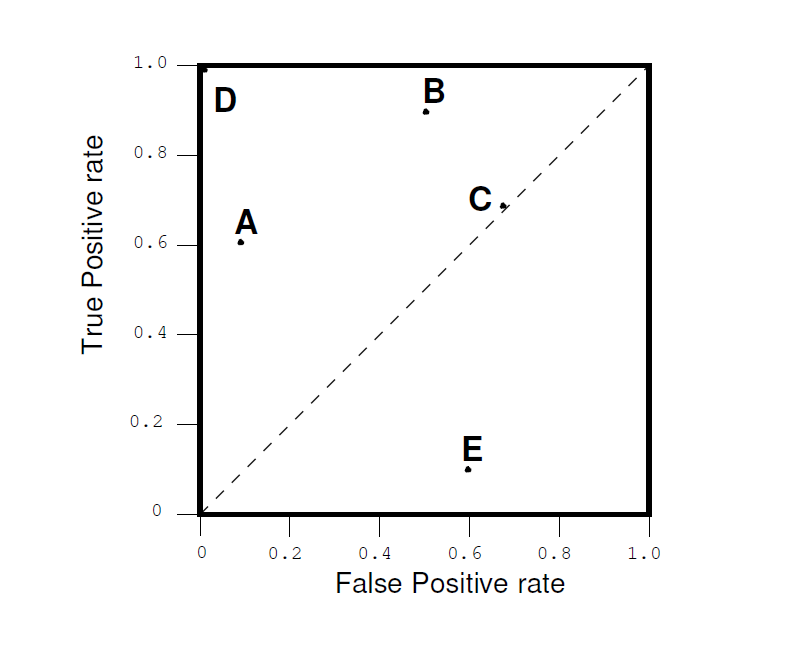
\includegraphics[scale=0.3]{roc-curve}
    \caption{ROC curve} \label{roc}
  \end{center}
\end{figure}

\subsection{Evaluation - Metrics}
The following table gives the metrics of the classifiers used in the previous chapter. We chose the optimum model for each type of classifier. The listed measures should be high for a good classifier, as seen from the table Logistic Regression performs the best for each metric. Since in our problem predicting the survival rate is important, the metrics with Negatives are more valuable, namely Specificity. Based on this we can say Random Forest and Decision Trees  perform in the same way. Between Naive Bayes and SVM, Naive Bayes is better since it has higher Specificity which means it predicts negatives better. Similarly between SVM and Decision Trees, latter performs better.
\begin{table}[h]
    \begin{tabular}{llllll}
    Measure              & Logistic Regression & Naive Bayes & SVM  & Decision Trees & Random Forests \\ \hline
    Precision            & 0.87                & 0.85        & 0.81 & 0.82           & 0.83           \\
    Recall / Sensitivity & 0.91                & 0.87        & 0.95 & 0.92           & 0.92           \\
    Specificity          & 0.77                & 0.74        & 0.62 & 0.67           & 0.68           \\
    Accuracy             & 0.86                & 0.82        & 0.82 & 0.83           & 0.83           \\
    \end{tabular}
    \caption{Performance Metrics of Models}
\end{table}

\subsection{Evaluation - ROC Curve}

\begin{figure}[h]
  \begin{center}
  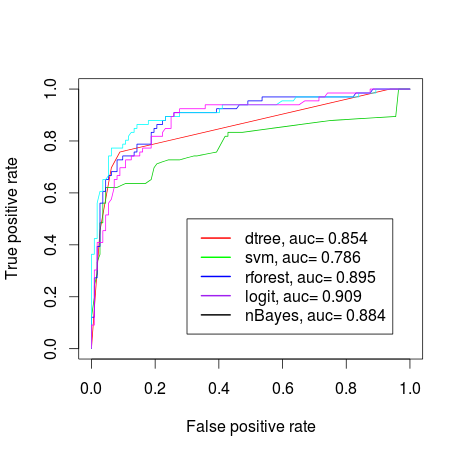
\includegraphics[scale=0.5]{rocr}
  \caption{ROC curves for models and their Area under the Curve (auc)} \label{rocr}
  \end{center}
\end{figure}

The obtained curves in Figure\ref{rocr} corroborate the evidence from the table. The accuracy of the classifier can be determined by computing the area under it's ROC curve. The area under the curve(\emph{auc}) was calculated for all five classifiers and the results are included in \ref{rocr}. It can be observed that the classifier based on logistic regression has performed the best, while the SVM-based classifier has the worst performance for the given dataset in terms of \emph{auc} as well.
\end{document}
